\documentclass{article}
% pre\'ambulo

\usepackage{lmodern}
\usepackage{float}
\usepackage[T1]{fontenc}
\usepackage{graphicx}
\usepackage[spanish,activeacute]{babel}
\usepackage{mathtools}

\title{Algoritmos de reconstrucci\'on}
\author{Luis A. Escamilla}



\begin{document}
\maketitle
% cuerpo del documento

  
    \maketitle
    \begin{abstract}
      Aqu\'i va el abstract o resumen.
    \end{abstract}









\section*{Estad\'istica Bayesiana}

Para entender c\'omo se har\'a la reconstrucci\'on se necesita entender un poco de estad\'istica bayesiana. En espec\'ifico se necesita saber sobre cadenas de Markov y sobre el m\'etodo de Cadenas de Markov Monte Carlo (MCMC por sus siglas en ingl\'es). Por lo que se dar\'a una breve introducci\'on a la estad\'istica bayesiana y sus conceptos antes de discutir MCMC.

\subsection*{Conceptos, definiciones y ejemplos}

En estad\'istica bayesiana las probabilidades se encuentran en la mente, no en el mundo. Esta frase nos da una peque\~na noci\'on sobre el c\'omo se trabaja con estad\'istica bayesiana. Por ejemplo, supongamos que alg\'un participante de un programa de televisi\'on debe contestar una pregunta de opci\'on m\'ultiple, si hay 4 opciones, digamos que son incisos a, b, c y d, y la persona no tiene idea de cu\'al sea la respuesta correcta, entonces esa persona tiene 1/4 de probabilidades de escoger la opci\'on correcta si elige al azar. Ahora supongamos que se le permite pedir ayuda a otra persona para responder la pregunta, si esta persona le dice ``creo que es el inciso $a$'' entonces el participante podr\'ia inclinarse en creer que el inciso $a$ es la respuesta correcta, lo que har\'ia que la probabilidad de $a$ aumente en la mente del participante. Si dejan que pida ayuda a una tercera persona y \'esta le responde tambi\'en que cree que es el inciso $a$ entonces el participante estar\'a a\'un m\'as seguro de que $a$ es la respuesta correcta. 

Analizemos este peque\~no ejemplo que acabamos de plantear. El participante ten\'ia 4 opciones iniciales pero no estaba seguro de cu\'al era la correcta, al recibir ayuda de la segunda persona recibi\'o nueva informaci\'on sobre el problema, lo que caus\'o una inclinaci\'on hacia una de las 4 opciones, aumentando su probabilidad. Al hacerle la pregunta a la tercer persona y responder lo mismo que la segunda entonces aument\'o a\'un m\'as la probabilidad de que $a$ fuese la respuesta correcta. Este peque\`no ejemplo nos da la noci\'on de un concepto importante para entender la estad\'istica bayesiana: \textbf{al recibir nueva informaci\'on sobre alg\'un fen\'omeno para el que se tienen varias hip\'otesis que intenten explicar su comportamiento, cada una de ellas con su propia probabilidad de ser cierta, se deben actualizar las probabilidades de que alguna de estas hip\'otesis sea la correcta con base en la informaci\'on que se recibi\'o.} En el ejemplo de arriba las hip\'otesis son las 4 posibles respuestas, el fen\'omeno es la pregunta y la nueva informaci\'on recibida es la respuesta de las 2 personas a las que se les pidi\'o ayuda. Al pedirles ayuda se actualizaron las probabilidades de cada una de las 4 posibles respuestas pues la ``nueva informaci\'on'' indicaba que $a$ ten\'ia mayor probabilidad de ser correcta que las otras 3. 

Ahora veamos otro ejemplo en el que emplearemos n\'umeros para poder dejar en claro la base de toda la estad\'istica bayesiana: la \textbf{regla de Bayes.} Supongamos que tenemos una bolsa con 2 bolas dentro, una de ellas estamos completamente seguros de que es negra, pero la otra podr\'ia ser negra o blanca. Esta situaci\'on nos presenta dos casos a los que llamaremos \textbf{hip\'otesis} NN (dos bolas negras) y NB (una bola negra y una blanca). En principio ambos casos son igualmente probables, por lo que su probabilidad inicial es $0.5$. Si lo acomodamos en una \textbf{caja de Bayes} quedar\'a mejor representado:

\begin{center}
\begin{tabular}{ |c|c|c|c|c| } 
\hline
Hip\'otesis & anterior & verosimilitud &  h  & posterior \\
\hline
NN & 0.5 & \quad &  & \\
NB & 0.5 &  &  & \\
\hline
Total: & 1 &  &  & \\
\hline
\end{tabular}
\end{center}
siendo $h=anterior \times verosimilitud$. Nuestras hip\'otesis tienen una cierta probabilidad inicial (anterior) que puede ser escogida dependiendo de las circunstancias. Si ahora procedemos a sacar una bola de la bolsa y resulta ser negra podremos empezar a calcular la $verosimilitud$ (likelihood en ingl\'es), que es un tipo muy especial de probabilidad. La verosimilitud se define como: probabilidad de haber calculado los datos suponiendo que la hip\'otesis fuese verdad. En este caso los ``datos calculados'' es el haber sacado una bola negra de la bolsa, si NN fuese la hip\'otesis correcta entonces la probabilidad de sacar una bola negra es 1, mientras que en NB es 0.5, por lo que la tabla queda:

\begin{center}
\begin{tabular}{ |c|c|c|c|c| } 
\hline
Hip\'otesis & anterior & verosimilitud &  h  & posterior \\
\hline
NN & 0.5 & 1   & 0.5  & \\
NB & 0.5 & 0.5 & 0.25 & \\
\hline
Total: & 1 &  & 0.75  & \\
\hline
\end{tabular}
\end{center}
Pero a\'un nos falta calcular el $posterior$. El $posterior$ es la ``nueva probabilidad'' dados los datos o informaci\'on nueva y no es m\'as que obtener la proporci\'on de la $verosimilitud$ de cada hip\'otesis con la suma de todas las verosimilitudes (b\'asicamente lo normalizamos para obtener nuevas probabilidades que sumen 1). Entonces nuestra caja de Bayes est\'a terminada:

\begin{center}
\begin{tabular}{ |c|c|c|c|c| } 
\hline
Hip\'otesis & anterior & verosimilitud &  h  & posterior \\
\hline
NN & 0.5 & 1 & 0.5 & 0.667 \\
NB & 0.5 & 0.5 & 0.25 & 0.333 \\
\hline
Total: & 1 &  & 0.75 & 1 \\
\hline
\end{tabular}
\end{center}
Observemos que ahora NN tiene mayor probabilidad que NB pues hay mayor probabilidad de sacar una bola negra en NN en NB, haciendo que NN sea la hip\'otesis m\'as probable luego de realizar la ``medici\'on''.

Este ejemplo nos ayuda a sentar las bases para definir la \textbf{regla de Bayes}:

\begin{equation}
P(H\vert D)=\frac{P(D\vert H)P(H)}{P(D)}
\end{equation}
siendo $H$ la hip\'otesis, $D$ los datos y:

\begin{itemize}
\item $P(H\vert D)$: probabilidad posterior. Qu\'e tan probable es que H sea cierto dado que obtenemos D. 
\item $P(H)$: probablidad anterior. Qu\'e tan probable es que H sea cierto antes de haber observado D.
\item $P(D\vert H)$: verosimilitud. Qu\'e tan probable es que observemos D si H es cierto.
\item $P(D)$: verosimilitud marginal. Probabilidad de observar D sin saber si H es verdad o no.
\end{itemize}
y si generalizamos para $N$ hip\'otesis:


\begin{equation}
P(H_i \vert D)=\frac{P(D\vert H_i)P(H_i)}{P(D)},\quad i=1,2,..., N
\end{equation}
\begin{equation}
P(D)= \sum_{i=1}^{N} P(H_i)P(D\vert H_i)
\end{equation}
y esto podemos ponerlo en una caja de Bayes como:

\begin{center}
\begin{tabular}{ |c|c|c|c|c| } 
\hline
Hip\'otesis & anterior & verosimilitud &  h  & posterior \\
\hline
$H_1$ & $P(H_1)$ & $P(D\vert H_1)$ & $P(H_1)\times P(D\vert H_1)$ & $P(H_1\vert D)$ \\
$H_2$ & $P(H_2)$ & $P(D\vert H_2)$ & $P(H_2)\times P(D\vert H_2)$ & $P(H_2\vert D)$ \\
... & ... & ... & ... & ... \\
\hline
Total: & 1 &  & $P(D)$ & 1 \\
\hline
\end{tabular}
\end{center}

\subsection*{Estimaci\'on de par\'ametros}

La estad\'istica bayesiana tambi\'en se puede utilizar para la estimaci\'on de par\'ametros de ciertas distribuciones. Para demostrarlo haremos un ejemplo.

Supongamos que un estudiante acaba de cambiarse de estado y est\'a averiguando c\'omo ir a nueva universidad tomando el transporte p\'ublico. Al investigar un poco se da cuenta de que tiene que tomar un cami\'on en cierta calle y \'este lo llevar\'a a su universidad. En la primer semana toma 5 camiones, uno por d\'ia, y 2 de estos 5 camiones lo llevan a su universidad mientras que los otros 3 lo llevan m\'as lejos y tiene que caminar m\'as para poder llegar a la universidad. Este estudiante quiere entonces calcular el porcentaje de camiones que lo dejan cerca. Vamos a atacar este problema con estad\'istica bayesiana.

Definamos a la proporci\'on de camiones que lo dejan cerca como $\theta$, dado que es una proporci\'on entonces $0\leq \theta \leq 1$. En principio $\theta$ puede tomar cualquier valor entre 0 y 1, pero por ahora lo restringiremos a tomar valores en intervalos de 0.1, esto nos da 11 hip\'otesis, cada una con probabilidad igual $1/11$, escrbiendo esto en una caja de Bayes:

\begin{center}
\begin{tabular}{ |c|c|c|c|c| } 
\hline
Hip\'otesis de $\theta$ & anterior & verosimilitud &  h  & posterior \\
 & $p(\theta)$ & $p(x\vert \theta)$ & $p(\theta)p(x\vert \theta)$ & $p(\theta\vert x)$ \\
\hline
0   & 0.0909 &  &  &  \\
0.1 & 0.0909 &  &  &  \\
0.2 & 0.0909 &  &  &  \\
0.3 & 0.0909 &  &  &  \\
0.4 & 0.0909 &  &  &  \\
0.5 & 0.0909 &  &  &  \\
0.6 & 0.0909 &  &  &  \\
0.7 & 0.0909 &  &  &  \\
0.8 & 0.0909 &  &  &  \\
0.9 & 0.0909 &  &  &  \\
1   & 0.0909 &  &  &  \\
\hline
Total: & 1 &  &  &  \\
\hline
\end{tabular}
\end{center}
Aqu\'i se define $x$ como el n\'umero de \'exitos (n\'umero de camiones que si dejan al estudiante cerca de su escuela) de un total $N$ de repeticiones. Si hay $N$ repeticiones de un experimento ``aleatorio'' con probabilidad $\theta$ de que ocurra $x$ veces el evento buscado entonces podemos expresar su funci\'on de probabilidad como una funci\'on binomial:

\begin{equation}
p(x\vert \theta) = \frac{N!}{x!(N-x)!} \theta^x (1-\theta)^{N-x}.
\end{equation}
Esta funci\'on nos dice la distribuci\'on de probabilidad de $x$ dado $\theta$. Para este ejemplo $N=5$ y $x=2$. Esta distribuci\'on nos da entonces la verosimilitud para cada $\theta$, teniendo la verosimilitud podemos calcular tanto $h$ como la probabilidad posterior, entonces la caja de Bayes queda completa:

\begin{center}
\begin{tabular}{ |c|c|c|c|c| } 
\hline
Hip\'otesis de $\theta$ & anterior & verosimilitud &  h  & posterior \\
 & $p(\theta)$ & $p(x\vert \theta)$ & $p(\theta)p(x\vert \theta)$ & $p(\theta\vert x)$ \\
\hline
0   & 0.0909 & 0 & 0 & 0 \\
0.1 & 0.0909 & 0.0729 & 0.0066 & 0.0437 \\
0.2 & 0.0909 & 0.2048 & 0.0186 & 0.1229 \\
0.3 & 0.0909 & 0.3087 & 0.0281 & 0.1852 \\
0.4 & 0.0909 & 0.3456 & 0.0314 & 0.2074 \\
0.5 & 0.0909 & 0.3125 & 0.0284 & 0.1875 \\
0.6 & 0.0909 & 0.2304 & 0.0209 & 0.1383 \\
0.7 & 0.0909 & 0.1323 & 0.0120 & 0.0794 \\
0.8 & 0.0909 & 0.0512 & 0.0047 & 0.0307 \\
0.9 & 0.0909 & 0.0081 & 0.0007 & 0.0049 \\
1   & 0.0909 & 0 & 0 & 0 \\
\hline
Total: & 1 &  & 0.1515 & 1 \\
\hline
\end{tabular}
\end{center}
Ahora analizemos este ejemplo ahora que tenemos la caja de Bayes completa. Como observamos tenemos una funci\'on de densidad de probabilidad (69), y queremos saber el valor del par\'ametro $\theta$ dados los datos $x$ y $N$. En la tabla observamos que la probabilidad posterior mayor corresponde a (sin mucha sorpresa) $\theta=0.4$. Entonces es seguro decir que, dada la informaci\'on proporcionada, el valor del par\'ametro $\theta=0.4$ es el que mejor se ajusta a la informaci\'on. Esto tiene sentido, pues de los 5 camiones que pasaron, \'unicamente 2 lo dejaron en la escuela, y $\frac{2}{5}=0.4$.

Podemos reescribir la regla de Bayes para la estimaci\'on de par\'ametros. Como el t\'ermino $P(D)$ es un t\'ermino de normalizaci\'on podemos retirarlo para reescribir (69) como:

\begin{equation}
p(\theta\vert x) \propto p(\theta)p(x\vert \theta)
\end{equation}
o
\begin{equation}
posterior \propto anterior \times verosimilitud
\end{equation}

\subsection*{Prueba de hip\'otesis (selecci\'on de modelo)}

Como vimos en la secci\'on anterior, para realizar estimaci\'on de par\'ametros se necesitan las probabilidades posteriores de los valores posibles del par\'ametro. El valor del par\'ametro con una probabilidad posterior mayor se considera que es el valor que mejor se ajusta con los datos u observaciones.

Para realizar una prueba de hip\'otesis (o selecci\'on de modelo) en estad\'istica bayesiana sehace algo similar a una estimaci\'on de par\'ametros, pues los valores probables del par\'ametro son las hip\'otesis, pero un cierto int\'ervalo de valores tambi\'en pueden ser una hip\'otesis. 
Un ejemplo r\'apido de este caso ser\'ia, utilizando el ejemplo anterior de los camiones, decir que tenemos 2 hip\'otesis posibles, la nula $H_0$  y la alternativa $H_1$. Las definimos como:

\begin{center}
$H_0: \quad \theta \leq 0.5$

$H_1: \quad \theta > 0.5$
\end{center}
por lo que tenemos dos posibilidades, o el valor de $\theta$ est\'a de 0,5 hacia abajo o arriba de 0,5. Para obtener la probabilidad s\'olo tenemos que sumar las probabilidades posteriores de los valores independientes de $\theta$ seg\'un se ajusten a alguna de las dos hip\'otesis. Entonces

\begin{center}
$P(H_0\vert x)= P(\theta \leq 0.5 \vert x)=0.7467$

$P(H_1\vert x)= P(\theta > 0.5 \vert x)=0.2533$.
\end{center}
En este ejemplo se cumple que $P(H_0\vert x)+P(H_1\vert x)=1$ pues las hip\'otesis son m\'utuamente excluyentes (si ocurre $H_0$ es imposible que ocurra $H_1$). 


La regla de Bayes se cumple para ambas hip\'otesis, entonces

\begin{equation}
P(H_0\vert x)=\frac{P(x\vert H_0)P(H_0)}{P(x)}
\end{equation}
\begin{equation}
P(H_1\vert x)=\frac{P(x\vert H_1)P(H_1)}{P(x)}
\end{equation}
y de aqu\'i obtenemos la odds form de la regla de Bayes

\begin{equation}
\frac{P(H_0\vert x)}{P(H_1\vert x)}=\frac{P(x\vert H_0)}{P(x\vert H_1)}\times \frac{P(H_0)}{P(H_1)}.
\end{equation}
donde a $\frac{P(x\vert H_0)}{P(x\vert H_1)}$ se le llama \textbf{factor de Bayes}, el cu\'al nos dice qu\'e tan probable es $H_0$ con respecto a $H_1$.


\subsection*{Cadenas de Markov}

Para explicar la reconstrucci\'on que se utilizar\'a hace falta explicar un poco un proceso estoc\'astico conocido como \textbf{Cadena de Markov}. Pero primero unas definiciones importantes:

\begin{itemize}
\item Proceso estoc\'astico: proceso que pretende describir la evoluci\'on temporal de alg\'un fen\'omeno aleatorio.
\item Propiedad de Markov: propiedad de los procesos estoc\'asticos que consiste en su ausencia de memoria, esto significa que la distribuci\'on de probabilidad de estados futuros del proceso depende \'unicamente del estado presente (ninguno de los estados anteriores al presente afectan esta distribuci\'on de eventos futuros, por esto se dice que tiene ausencia de memoria, pues no ``recuerda''los pasos anteriores al actual o presente). Si un proceso tiene esta propiedad se le llama \textit{proceso de Markov}.

\end{itemize} 

Usando estas definiciones ahora podemos definir una cadena de Markov.

\begin{itemize}
\item Cadena de Markov: proceso de Markov que describe una secuencia de posibles eventos represent\'andolos como ``pasos'' o ``eslabones''.
\end{itemize}
Ejemplos muy populares de procesos que pueden ser modelados por una cadena de Markov son los llamados \textit{caminantes aleatorios}.

Dado que las cadenas de Markov son un proceso de Markov cada paso que da la cadena es indiferente a todos los anteriores excepto por el paso en el que se encuentre en ese momento.

Las cadenas de Markov pueden representarse como un diagrama de distintos estados. Pongamos un ejemplo, imaginemos que Pepito realiza alguna de las siguientes 3 actividades todos los d\'ias: correr, dormir o comer helado y por alguna raz\'on un amigo suyo realiz\'o una estad\'isica de su comportamiento. El amigo descubri\'o que si Pepito dorm\'ia, al d\'ia siguiente ten\'ia una probabilidad de 0,6 de correr, una probabilidad de 0,2 de comer helado y una de 0,2 de volver a dormir. Si Pepito com\'ia helado entonces era 0,7 de correr, 0,1 de comer helado de nuevo y 0,2 de dormir, y si corr\'ia entonces era 0,6 de volver a correr al d\'ia siguiente, 0,1 de dormir y 0,3 de comer helado. Esta informaci\'on se puede representar de manera m\'as f\'acil en un diagrama de un proceso de Markov como el de la Figura 1.


\begin{figure}[H]
\begin{center}
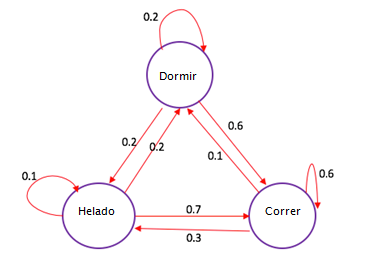
\includegraphics[scale=0.8]{cadenamarkovejemplo}
\caption{Diagrama que representa el proceso de Markov.}
\end{center}
\end{figure}
Si la cadena de Markov comenzase en el estado \textit{dormir} podemos ver en el diagrama la probabilidad que tienen los 3 estados de ser el siguiente paso en la cadena.



\subsection*{Cadenas de Markov Monte Carlo (MCMC)}

Se le llama \textit{Monte Carlo} de manera general a alguna t\'ecniva computacional que utilice n\'umeros aleatorios. Un tipo de Monte Carlo es MCMC, y un topo de m\'etodo MCMC es el algoritmo Metropolis-Hastings. Este algoritmo nos da una manera de construir una cadena donde los valores de alg\'un par\'ametro con probabilidades posteriores mayores aparezcan de manera m\'as frecuente en la cadena que los valores con probabilidades posteriores menores, pero no hace que sea imposible que los valores con probabilidades menores ocurran, por lo que estar\'an presentes en la cadena pero con menos frecuencia.

De manera sencilla, el algoritmo funciona de la siguiente manera:

\begin{enumerate}
\item Se comienza en alg\'un estado $\theta$.
\item Se genera una propuesta $\theta'$ para el siguiente paso.
\item Si la $h'=posterior \times verosimilitud$ de $\theta'$ es mayor que la $h$ del estado actual entonces se da el paso hacia $\theta'$ en la cadena y \'este ser\'a el nuevo estado actual de la cadena, se reinicia el proceso con $\theta'$ como el nuevo estado inicial. 
\item Si $h'$ es menor entonces se propone una probabilidad m\'inima $h'/h$ y se genera un n\'umero aleatorio entre 0 y 1, si el n\'umero generado es mayor o igual a $h'/h$ entonces se da el paso y $\theta'$ ser\'a el nuevo estado actual en la cadena, se reinicia el proceso con $\theta'$ como nuevo estado inicial, pero si el n\'umero generado es menor que $h'/h$ entonces se rechaza la propuesta $\theta'$ y se reinicia el proceso.
\end{enumerate}

Si observamos bien el paso 4 del algoritmo podemos observar que $h'/h$ es la ec. (74), por lo que el algoritmo Metropolis-Hastings es una forma de realizar comparaciones entre hip\'otesis. Cada hip\'otesis tiene una cierta probabilidad de ser cierta. Lo que se pretende lograr con MCMC es correr una cadena lo suficientemente larga como para...








\end{document}